\newcommand{\roborta}{Roborta\xspace}
\section{\roborta vs.\ La Luz Fair (Un Ejemplo Motivador)} \label{sec:mot_example_fair}

\begin{figure}[t]
\centering
\begin{minipage}[t]{.47\textwidth}
{\fontsize{7.6}{7.6}\selectfont\ttfamily
\begin{tabbing}
x\=xxxxxxxxxx\=xxxxxx\=xxx\=xxxx\=xxx\=xxxx\= \kill    
module \roborta\_vs\_the\_light\\[1ex]
\>col : [0..WIDTH] init 0; \\
\>row : [0..LENGTH] init 0; \\
\>light : [0..3] init 0; \>\>\>\> // color de luz actual \\%[1ex]
\>                   \>\>\>\>// 0: rojo (turno de la luz) \\%[1ex]
\>                   \>\>\>\>// 1: amarillo (\roborta se mueve lateralmente) \\%[1ex]
\>                   \>\>\>\>// 2: verde (\roborta se mueve hacia delante) \\%[1ex]
\>                   \>\>\>\>// 3: apagado (falla la luz) \\[1ex]
%\> // board allowed movements: 0:left, 1:both, 2:right \\[1ex]
\> // light moves \\[1ex]
\>[l\_y] (light=0) \> \>-> \>(1-Q) : (light'=1) + Q : (light'=3);\\[1ex]
\>[l\_g] (light=0) \> \>-> \>(1-Q) : (light'=2) + Q : (light'=3);\\[1ex]
%% \>[l\_y] (light=0) \> \>-> \>(1-Q) : (light'=1) + \\
%% \> 					 \> \> \> Q : (light'=3);\\[1ex]
%% \>[l\_g] (light=0) \> \>-> \>(1-Q) : (light'=2) + \\
%% \> 					 \> \> \> Q : (light'=3);\\[1ex]
\> // \roborta moves \\[1ex]
\>[r\_l]  ((light=1) | (light=3)) \& (MOVES[col,row] <= 1)  \\
\>                    \>\>-> \>(1-P) : (light'=0) \& (col'=(col-1)\%WIDTH) + \\       
\>                     \>\>\>  P : (light'=0) ; \\[1ex]

\>[r\_r] ((light=1) | (light=3)) \& (MOVES[col,row] >= 1)\\
\>                    \>\>-> \> (1-P) : (light'=0) \& (col'=(col+1)\%WIDTH) + \\
\>                     \>\>\> P : (light'= 0); \\[1ex]
\>[r\_f] ((light=2) | (light=3)) \& (row < LENGTH) \\
\>                    \>\>-> \> (1-P) : (light'=0) \& (row'=row+1)  + \\
\>                     \>\>\> P : (light'= 0);\\[1ex]
endmodule\\[-5ex]
\end{tabbing}}
\end{minipage}
\vspace{0.5cm}
\caption{Modelo para el Juego de Roborta vs la Luz fair} \label{fig:robot_game_model}
\end{figure}

Consideremos el siguiente escenario. El robot \roborta navega por una cuadrícula de $4 \times 4$ celdas. Hay una señal de luz
determinar los posibles movimientos del robot: si la luz es amarilla, debe moverse hacia los lados (en una celda del borde, \roborta puede envolverse hacia el otro lado); si el semáforo está en verde, debe avanzar hacia delante; si la luz es roja, no puede realizar ningún movimiento; si la luz está apagada, el robot puede moverse libremente hacia los lados o hacia adelante. La señal de luz y \roborta cambian sus estados por turnos. Se asocia una recompensa (no negativa) con cada ubicación de la cuadrícula. Además, los movimientos laterales pueden restringirse a una sola dirección en algunos lugares.
Además, consideramos posibles fallas en el comportamiento del robot y la luz. Si \roborta falla, pierde su turno para moverse, y si falla la luz, se apaga sola. Las fallas ocurren con una probabilidad dada. El objetivo de \roborta es recolectar tanta recompensa como sea posible. Por el contrario, la luz apunta a minimizar este valor.

La especificación de este juego se captura en la Fig.~\ref{fig:robot_game_model} (usando la notación similar a {\Prism} \cite{DBLP:conf/cav/KwiatkowskaNP11}).
%% %
%% \begin{wrapfigure}[11]{r}{52mm}
%% \vspace{-5mm}
%% {\fontsize{6.6}{6.6}\selectfont\ttfamily
%% \centering
%% 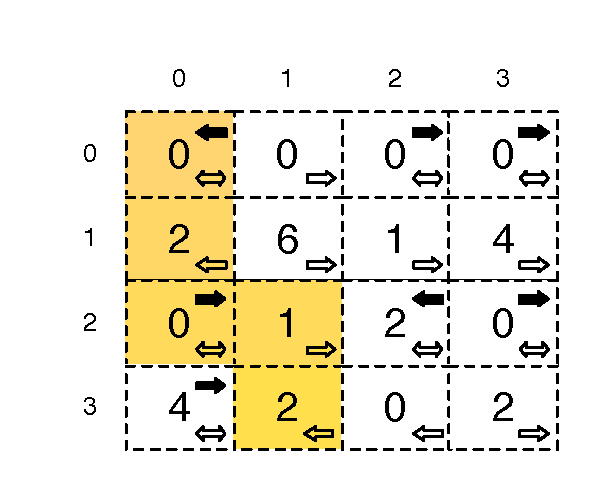
\includegraphics[scale=0.45]{Figs/robotMovesRewards.eps}\hspace{1em}\mbox{}}
%% \caption{A robot on a $4 \times 4$ grid} \label{fig:robot_game_grid}
%% \end{wrapfigure}
%% 
%% \noindent
En este modelo, \texttt{WIDTH} y \texttt{LENGTH} son constantes que definen la dimensión de la cuadrícula. \texttt{MOVES} es una matriz bidimensional que modela los posibles movimientos laterales en la cuadrícula (\texttt{0} permite que el robot se mueva solo hacia la izquierda, \texttt{1}, hacia cualquier lado y \texttt{2 }, solo a la derecha). Cuando la luz está en rojo (\texttt{light=0}) es el turno de la luz y puede escoger entre cambiar a amarillo (la transición etiquetada \texttt{l\_y}) o verde (la transición etiquetada \texttt{l\_g}). Observemis que cualquiera sea la elección, la luz puede fallar con probabilidad \texttt{Q}, en cuyo caso la luz se apaga (\texttt{light’=3}). Si la luz no está en rojo, entonces es el turno de Roborta. Si la luz está en amarillo (\texttt{light=1}) o está apagada (\texttt{light=3}), Roborta puede elegir moverse a la izquierda (\texttt{r\_l}) o a la derecha (\texttt{r\_r}), suponiendo que la matriz permite esos movimientos. Si la luz está en verde (\texttt{light=2}) o está apagada (\texttt{light=3}), Roborta puede elegir moverse hacia delante (en la figura sería hacia abajo), notemos que cuando \texttt{light=2} esta es a única alternativa. Al igual que la luz, cada elección de Roborta está sujeta a una probabilidad de falla (\texttt{P}), en cuyo caso, no puede realizar ningun movimiento y consume su turno (cambia el valor de \texttt{light} a 0). Vale la pena mencionar que omitimos en la Fig.~\ref{fig:robot_game_model} una matriz secundaria con las recompensas asignadas a cada posición.

%Las recompensas asignadas a cada ubicación de la cuadrícula se almacenan en una matriz llamada \texttt{REWARDS}.
La Figura~\ref{fig:robot_game_grid} muestra la asignación de recompensas a cada ubicación de la cuadrícula de $4 \times 4$, así como las restricciones de movimiento lateral (que se muestran en la parte inferior derecha de cada ubicación con flechas blancas).
El juego comienza en la ubicación $(0, 0)$ y se detiene cuando \roborta escapa por el final de la cuadrícula.


\begin{figure}
\centering
{\fontsize{6.6}{6.6}\selectfont\ttfamily
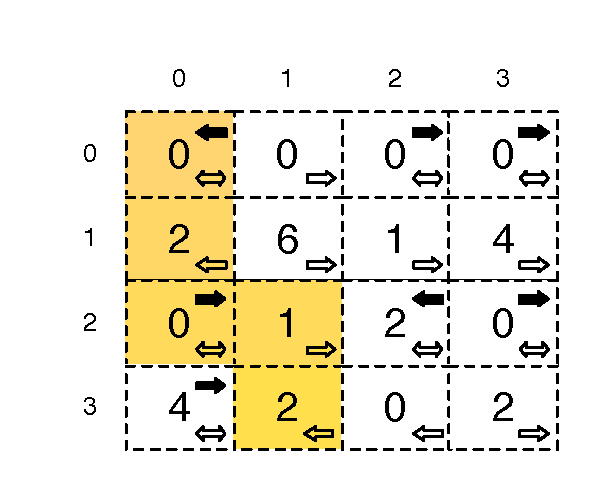
\includegraphics[scale=0.65]{Figs/robotMovesRewards.eps}\hspace{1em}\mbox{}}
\caption{\roborta en una matriz $4 \times 4$} \label{fig:robot_game_grid}
\end{figure}

Un escenario posible en este juego es el siguiente. \roborta comienza en la celda $(0,0)$ y, en un intento de minimizar las recompensas acumuladas por el robot, el entorno enciende la luz amarilla.
En aras de la simplicidad, asumimos que no hay fallas en la luz, es decir, $\texttt{Q}=0$.
Observemos que, si el ambiente juega siempre de esta manera (encendiendo la luz amarilla), entonces \roborta nunca alcanzará la meta y
el juego nunca terminaría. Este escenario ocurre cuando la luz juega de manera infair, es decir, una acción (la que enciende la luz verde) se habilita con infinita frecuencia, pero no se ejecuta con infinita frecuencia.
Suponiendo que el medio ambiente sea fair, podemos asegurar que finalmente se encenderá una luz verde, lo que permitirá que el robot avance.

Para el caso de \texttt{Q=0}, la mejor estrategia para \roborta cuando la luz es amarilla se muestra con flechas negras en la parte superior derecha de las celdas sin restricciones de movimiento.
% Como resultado, la mejor estrategia para lograr el objetivo del robot se puede observar en la parte resaltada de la cuadrícula en amarillo en
Como resultado, cuando ambos jugadores juegan sus estrategias óptimas, el camino tomado por \roborta para alcanzar la meta se puede observar en la Figura~\ref{fig:robot_game_grid} en la parte resaltada en amarillo de la cuadrícula. En la Sección \ref{sec:experimental_eval_fair}, evaluamos este problema experimentalmente con diferentes
configuraciones de este juego.